%!TEX root = main.tex
\section{Design Guidelines\label{sec:guidelines}}

\subsection{Search-Browse Paradigm}

\subsection{Top-down approaches}
\subsection{Bottom-up approaches}

\begin{figure*}[ht!]
\centering
\vspace{-15pt}
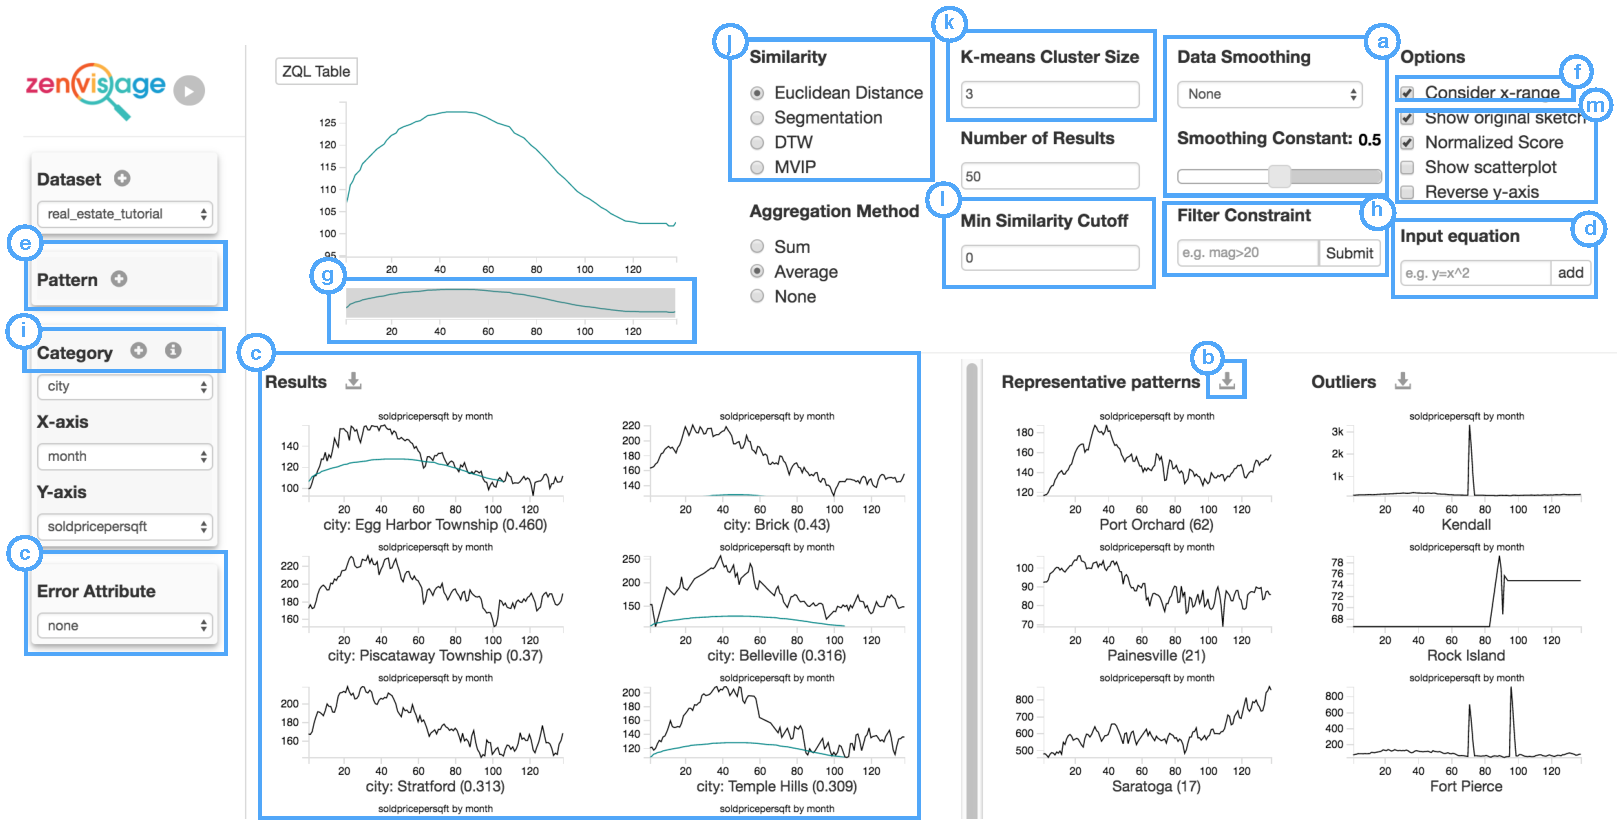
\includegraphics[width=\linewidth]{figures/newZV.pdf} %5.5
\vspace{-5pt}\caption{Our VQS after participatory design, which includes: the ability to preprocess via (a) interactive smoothing; (b, c) the ability to export data outputs ; querying functionalities via (d) equations and (e) patterns; query specification mechanisms including (f) x-range invariance, (g) x-range selection and filtering, (h) Filtering, and (i) Dynamic class creation; (j, k, l) system parameter options; (m) visualization display options. Prior to the participatory design, \zv only included a single sketch input with no additional options. \zv also displayed representative patterns and outlier patterns, as shown in Figure~\ref{oldZV}.}
\label{zvOverview}
\vspace{-14pt}
\end{figure*}



% \subsection{Characteristic Challenges for VQSs}
% \par Based on the participatory design and evaluation study, we learn about the characteristic challenges that these use cases pose on existing VQSs.
% \par In the astronomy use case, the participants knew the patterns they are looking for, but the patterns are hard to specify and find. The main challenge for the VQS involves finer specification of sketched patterns, such as amplitude and width of the peak and noise level tolerance for defining a pattern match. In the material science use case, the participants are able to identify interesting relationships between physical variables when they see it, but they are not sure what patterns to look for to begin with. Similarly, for the genetics participants, they do not have a preconceived knowledge of what they want to search for in the dataset. They use clustered results to jumpstart their further queries